% section on the physics case


The core of the physics case for the ILC is to make high-precision
 measurements of the properties of the Higgs boson.    The Higgs
 field has a central role in 
 the SM.  It is responsible for the masses of all known
 elementary particles.
  It is also responsible for those aspects of the SM that are
 hardest to  understand----the
presence of spontaneous gauge symmetry breaking, the  hierarchy of quark and lepton masses, and the appearance of flavor mixing and $CP$ violation in weak 
interactions.
If we wish to learn more about these features of the fundamental laws of nature, an obvous course is to measure the Higgs boson as well as we are able.  We will argue in this section and the succeeding ones that ILC will be able to determine the mass of the Higgs boson to a part in $10^4$ and the major couplings of the Higgs boson to than 1\% accuracy.   This will qualitatively sharpen the picture of the Higgs boson that we will obtain even from the high-luminosity stage of the LHC. 

This set of measurements, and other measurements available for the first time at the ILC, will open new paths in the search for new fundamental interactions beyond the SM. 
Though the SM seems to account for all elementary particle phenomena observed up to now, it is manifestly incomplete.   It not only does not answer but actually is incapable of answering the questions posed in the previous paragraph.  It also cannot address basic facts about the universe in the large, in particular, the excess of matter over antimatter and the origin of the cosmic dark matter.  To make progress, we need observational evidence from particle physics of violations of the SM.  These will provide clues that can show the way forward.

Up to now, we have sought evidence for new interactions from direct searches for new particles at LEP, the Tevatron, and the LHC, from measurements of the $W$ and $Z$ bosons, and from searches for anomalies in flavor physics.  We are now approaching the limits of these techniques with current particle physics facilities.  The ILC will 
extend our search capabilities in precision measurements of $W$ boson couplings and fermion pair production, and will provide new opportunites for the direct discovery of new particles.  But, most of all, it will open a completely new road through the thorough, high-precision study of the Higgs boson. 


\subsection{Mysteries of the Higgs boson}

We often hear from our colleagues that the Higgs boson, as observed at the LHC, is an uninteresting particle, since it conforms so well to the expectations from the SM.   In fact, aside from our knowledge of the Higgs boson mass, the measurements make so far at the LHC tell us almost nothing about the true nature of this particle.   We now 
explain this statement, and, in the process, clarify the requirements for measurements of the Higgs boson couplings that can give insight into physics beyond the SM. 

New physics can correct the Higgs boson couplings in many ways.  However, in all cases, the size of the corrections is limited by the Decoupling Theorem, enunciated by Haber in \cite{Haber:1994mt}:    If the new particles that modify the SM have minimum mass $M$, then  the corrections to the SM predictions for the Higgs boson couplings are of size 
\beq 
              a \,     m_H^2 / M^2   \  .
\eeqn
where the coefficient $a$ is of order 1.   The exclusions of new particles through searches at the LHC suggest that $M$ is at least close to 1~TeV.   Then the effects of  new physics are limited to the few-percent level.   We will illustrate this result with explicit models in the next subsection.

The proof of the theorem is simple and illustrative.   It can be shown that the SM is actually the most general renomalizable quantum field theory with $SU(3)\times SU(2)\times U(1)$ gauge symmetry and the known particle content.   If we add new particles with masses of $M$ and above, we can assess their influence on the Higgs boson by integrating them out of the theory.  This adds to the Lagrangian a set of new terms with the SM symmetries.   The terms in the new Lagrangian  can be organized by their operator dimension 
as 
\beq 
   {\L}  =  {\L}_{SM} + {1\over M^2} \sum_i\,  c_i \O_{6i} + {1\over M^4 } \sum_j\,  d_j\O_{8j} + \cdots
\eeq{geneffL}
where $\L_{SM}$ is the SM Lagrangian with modified parameters, $\O_{6i}$  are operators of dimension 6, $\O_{8j}$ are operators of dimension 8, \etc.   The shifts in the SM parameters are not observable, since these parameters are in any case fit to experiment.  Then the leading observable corrections are of order $M^{-2}$. 

This theorem has a striking consequence.  Instead of a model with a single Higgs doublet, as we have in the SM, nature could be providing  a model with two or more Higgs fields, composite Higgs fields, even a whole Higgs sector.  All of this possible complexity is hidden from us by the Decoupling Theorem. 

The theorem has an appealing corollary, though.   Since the SM is the most general renormalizable model, once its parameters are known, its predictions for the Higgs couplings are determined precisely.   These predictions do depend on measured SM parameters such as $m_b$, $m_c$, and $\alpha_s$, but  it is argued in \cite{Lepage:2014fla} that  
lattice QCD will determine these well enough to fix the SM predictions for Higgs to part-per-mil accuracy.   Then, if we can observe corrections to the SM predictures at the 1\% level, these corrections and the evidence that they give for new physics cannot hide.

\subsection{Examples of  new physics influence on the Higgs boson}
\label{subsec:newphysicofH}

Many models of physics beyond the SM illustrate the points made in the previous section. Here are some examples.   These examples point to  a goal of 1\% accuracy
for the measurement of Higgs boson couplings in the major decay modes.

Models with two Higgs doublets contain 5 physical Higgs particles: two  neutral $CP$-even states $h$, $H$,  a neutral $CP$-odd state $A$, and a pair of charged scalars $H^\pm$.  These states are mixed by two angles $\alpha, \beta$. The lighter
$CP$-even state $h$ is identified with the observed Higgs boson.  Its couplings to 
fermions depend on the mixing angles.   For example, in the ``Type II'' case, 
\beq
   g(Hb\bar b) = - {\sin\alpha\over \cos\beta}{m_b\over v}  \quad   g(Hc\bar c) =  {\cos\alpha\over \sin\beta}{m_c\over v}   \ .
\eeq{typeIIbcshift}
However, the mixing angles are connected to the masses in such a way that when the additional bosons become heavy, their effects in \leqn{typeIIbcshift} also become small,
\beq
     - {\sin\alpha\over \cos\beta} =  1 + \O({m_Z^2\over m_A^2}) \ ,
\eeqn
conforming to the Decoupling Theorem.   In Type II models, the $b$ and $\tau$ Yukawa couplngs are shifted together by about 5\% for $m_A = 500$~GeV, and by decreasing amounts when all of the additional bosons become heavier.

%%%%%%%%%%%%%%%%%%%%%%%%%%%%%%%%%%%%%%%%%%%%%%%%%%%%%%%%
\begin{figure}
\begin{center}
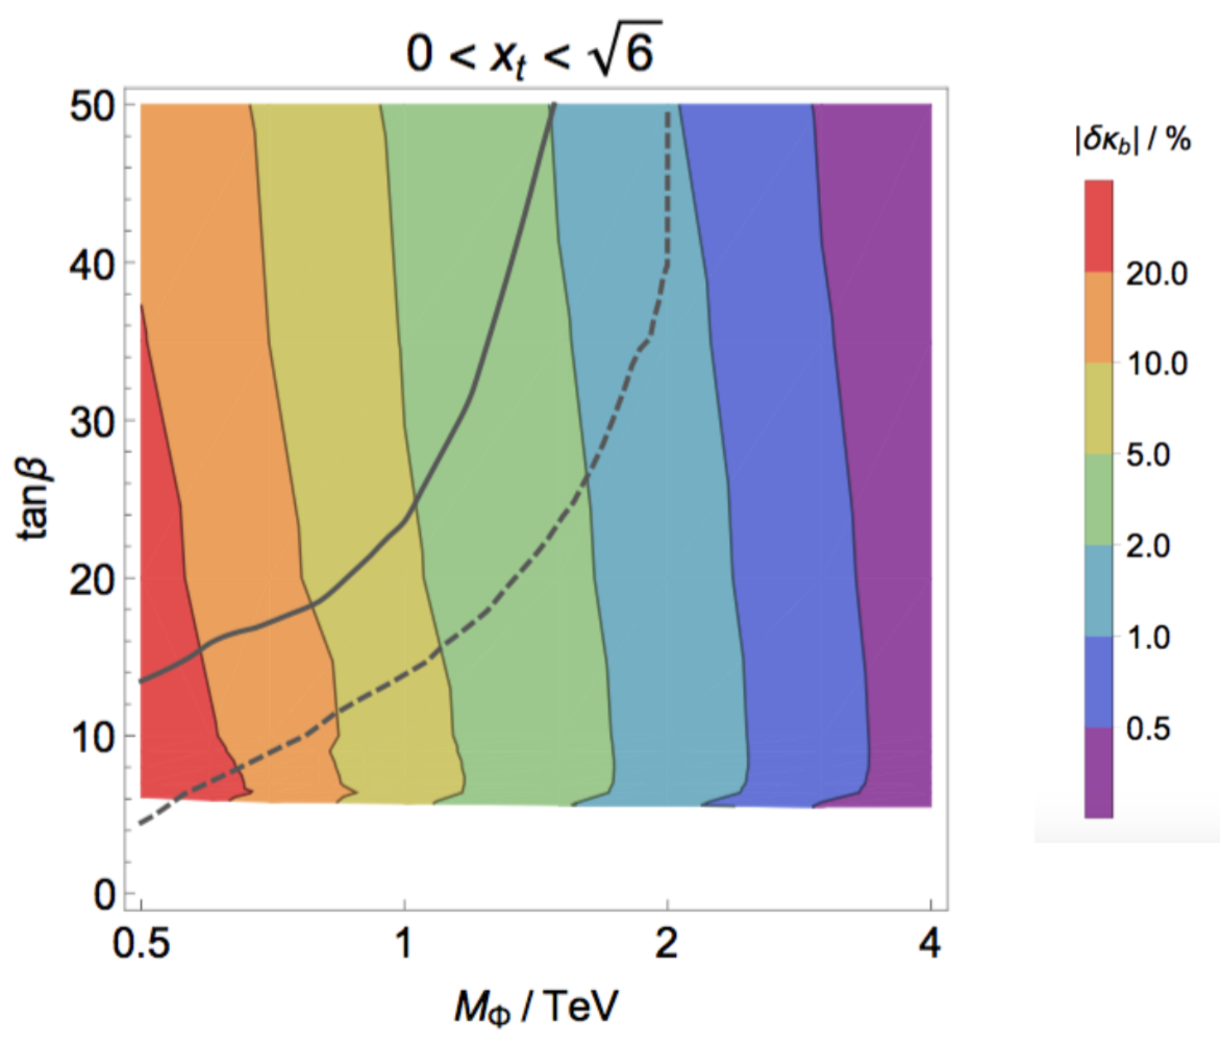
\includegraphics[width=0.90\hsize]{chapters/figures/WellsZhang.pdf}
\end{center}
\caption{Deviation from the SM prediction for the $Hb\bar b$ 
coupling over a parameter space of grand-unified SUSY models, from \cite{Wells:2017vla}.   
Models in the upper left-hand corner are excluded by current LHC searches.  
Models above the dashed line are expected to be excluded at the  HL-LHC. 
The color-code indicates the magnitude of the coupling deviation, in \%. }
\label{fig:WellsZhang}
\end{figure}
%%%%%%%%%%%%%%%%%%%%%%%%%%%%%%%%%%%%%%%%%%%%%%%%%%%%%%%%%%%%%%


Supersymmetry (SUSY) models contain Type II  two-Higgs-double sectors, but they also contain other effects that modify the Higgs boson couplings.   Mixing between the scalar partners of $b_L$ and $b_R$ can generate a shift of the $Hb\bar b$ coupling through loop diagrams.  The magnitude of this effect in 
grand-unified SUSY models is shown in 
Fig.~\ref{fig:WellsZhang}~\cite{Wells:2017vla}.   
Note that it is possible to have a large shift of the Higgs boson coupling for 
parameter values at which the SUSY particles are too
heavy to be discovered at the LHC.   Thus, the search for shifts in the Higgs couplings away from the SM predictions provides a method of searching for this new physics that is independent of, and largely orthogonal to, the direct search for SUSY particles.   Other surveys of this effect in \cite{Cahill-Rowley:2014wba,Kanemura:2015mxa}  confirm this idea.

SUSY models typically predict very small shifts of the $HWW$ and $HZZ$ couplings, but other types of models can affect these couplings directly.   Models in which the electroweak phase transition becomes first-order and allows baryogenesis at the weak scale often involve mixing of the Higgs field with a heavy singlet field.  This gives
\beq
           g(HWW) = {2m_W^2\over v} \cos^2\phi\approx  {2m_W^2\over v} (1 -\half \phi^2) \ ,
\eeq{scalarmixing}
where $\phi \sim  m_H/m_S$, and similarly for the $HZZ$ coupling~\cite{DiVita:2017eyz}   In composite models of the Higgs
 field, the Higgs field often appears as a Goldstone boson of a new strong interaction theory, giving a coupling modification by $(1- v^2/f^2)^{1/2}$, where $f$ is the Goldstone boson decay constant~\cite{Contino:2013kra}.  This effect is similar to that in \leqn{scalarmixing}.

Models of Higgs compositeness, ``Little Higgs'' models, and models with extra space dimensions all contain new heavy vectorlike fermions $T$.   Typically, these fermions obtain a fraction of their mass from the Higgs mechanism (perhaps by mixing with the top quark) that is of order $m_t^2/m_T^2$.   Then they induce corrections of this order to the loop-generated Higgs couplings $g(Hgg)$ and $g(H\gamma\gamma)$.  Corrections as large as 10\% can be generated in specific models~\cite{Han:2003gf}.   These same mixing and compositeness effects modify the $Ht\bar t$ coupling~\cite{Agashe:2004rs}.

An interesting picture emerges.   Almost all models of new physics generate corrections to the Higgs boson couplings.   Almost always, these corrections are small, below the 10\% level, in accord with the Decoupling Theorem.  However, in precision experiments that make these coupling deviations  visible, each type of new physics affects the Higgs couplings in different ways.  In general,
\begin{itemize}
\item The $Hb\bar b$ and $H\tau\tau$ couplings are sensitive to models with additional Higgs doublets.
\item The $Hb\bar b$ coupling is sensitive to heavy SUSY particles with left-right mixing.
\item The $HWW$ and $HZZ$ couplings are sensitive to mixing of the Higgs field with singlet fields, and to composite structure of the Higgs boson.
\item The $Hgg$ and $H\gamma\gamma$ are sensitive to models with new vectorlike fermions.
\item The $Ht\bar t$ coupling is sensitive to models with composite Higgs bosons and top quarks.
\end{itemize}

In each new physics model, the  deviations from the SM predictions for the Higgs couplings form a pattern.  With precision experiments, it is possible not only to discover the existence of new physics but also to read the pattern and gain clues as to the way forward.   A worked example of such model discrimination at the level of precision expected at the ILC  is presented in
Section~7 of  \cite{Barklow:2017suo}.


\subsection{Limitations of the LHC measurements on the Higgs boson}

Today, the LHC experiments are achieving 20\% uncertainties in their measurements of Higgs boson couplings.   Over the lifetime of the LHC, including its high-luminosity stage, these experiments will acquire a factor of 30 more data.   Shouldn't this lead to Higgs coupling measurements of the required high precision?  We believe that the answer to this question is no.   We give a high-level argument here. A detailed comparison of the expected ILC capabilities with those of the high-luminosity LHC will be presented in Sec.~\ref{subsec:higgs:ilclhc}.

We find three points relevant to this comparison.  First, the measurement of Higgs boson 
decays at the LHC is extremely challenging because of the difficulty of distinguishing 
signal from background.
In the two decay modes in which the Higgs boson was discovered, $H\to \gamma\gamma$ and $H\to 4\ell$, Higgs events are apparent, because all products of the Higgs are observed and the Higgs mass can be reconstructed with high accuracy.  Unfortunately, these modes correspond to tiny branching ratios,  0.2\% and 0.02\% of Higgs decays, respectively.  For more typical decay  modes, Higgs boson decay events have no obvious differences in appearance from SM background reactions with larger rates.   For example, $H\to WW\to e\nu \mu \nu $ events differ from $q\bar q\to WW \to  e\nu \mu \nu $ events only in subtle features of the lepton momentum distributions.  To discover the Higgs boson in one of the major channels, the LHC experiments start from samples that are 10:1 background to signal in the highest significance regions.  (For $H\to b\bar b$, the ratio is 20:1.) They then  extract the signal by multivariate analysis and the use of machine-learning classifiers.  It is already a
 triumph that ATLAS and CMS have been able to obtain significant observations. 

Measuring  the Higgs couplings with high precision is even more of a challenge.   It is currently beyond the state of the art to determine the efficiency  for the rejection of SM background events from these signal regions to 1\% accuracy.   The residual background events must be subtracted from the Higgs signal, and so this 1\% would translate to a 10\% accuracy on the Higgs $\sigma\times BR$ or a 5\% error on the coupling. To go beyond this level is truly daunting.  Nevertheless, the studies reported in the HL-LHC Yellow Book~\cite{Cepeda:2019klc} give reasons for optimism and cite goals of 2-4\%  for Higgs coupling uncertainties.

This brings us to the secoind point.  As we have emphasized already, the modifications of the Higgs boson couplings from new  physics are expected to be small.  In the previous section, we have argued that new physics interactions typically  affect specific
Higgs boson couplings at a level of 5\% or smaller.  A 2\% measurement of such a coupling  
would not meet the $3\sigma$ criterion for positive evidence of new physics.

Finally, one must take into account that the HL-LHC measurements will ultimately be limited by the systematic understanding of backgrounds  Any deviation in Higgs couplings observed at the LHC is  likely to be questioned (as, for example, the $t\bar t$ forward-backward asymmetry from the Tevatron was) without a clear means of confirming the result. 
One sometimes hears that the LHC can measure ratios of branching ratios with improved accuracy, but this statement is wrong for the major modes, since each mode has different backgrounds and requires its own dedicated analysis. 

 In contrast, as we will argue below, the observation of Higgs coupling deviations at the ILC at  250~GeV will be very robust.  It will be be statistics-limited,  and it can be confirmed by experiments at 500~GeV that bring in a new production reaction with an independent  data set. 


\subsection{$\ee\to ZH$}

The arguments just presented call out for a different way to measure Higgs boson couplings.   In this method, Higgs boson events should be apparent with a simple discriminator that can then be refined for high-accuracy $\sigma\times BR$ measurements.  Ideally, this method should identify Higgs boson events independently of the decay mode, allowing the measurement of the total cross section for Higgs production and the discovery of exotic and unanticipated Higgs decays.

This new method will be provided by the ILC.  It is the measurement of the reaction $\ee\to ZH$ at 250~GeV.   At an $\ee$ collider at this energy, it is true to a first approximation that any $Z$ boson observed with a lab energy of  110~GeV is recoiling against a Higgs boson.   The backgrounds to this signature (present at about 30\% of the signal level before cuts)  come from radiative $\ee\to Z\gamma$ and $\ee\to ZZ$, reactions that are well-understood and computed from electroweak theory at the 0.1\% level. 

The reaction $\ee\to ZH$ provides {\it tagged} Higgs decays.   Thus, events can be selected independently of the Higgs decay mode.  Then (1) the  total cross section for this reaction can be measured, giving a means of absolutely normalizing Higgs boson couplings; (2)  Higgs branching ratios can be measured  by counting, independently of the production cross section; and, (3)  exotic decay modes of the Higgs boson can be observed as products recoiling against the $Z$ tag.   Some event displays, from full 
simulation, are shown in Fig.~\ref{fig:HiggsEvents}. 

%%%%%%%%%%%%%%%%%%%%%%%%%%%%%%%%%%%%%%%%%%%%%%%%%%%%%%%%
\begin{figure}
\begin{center}
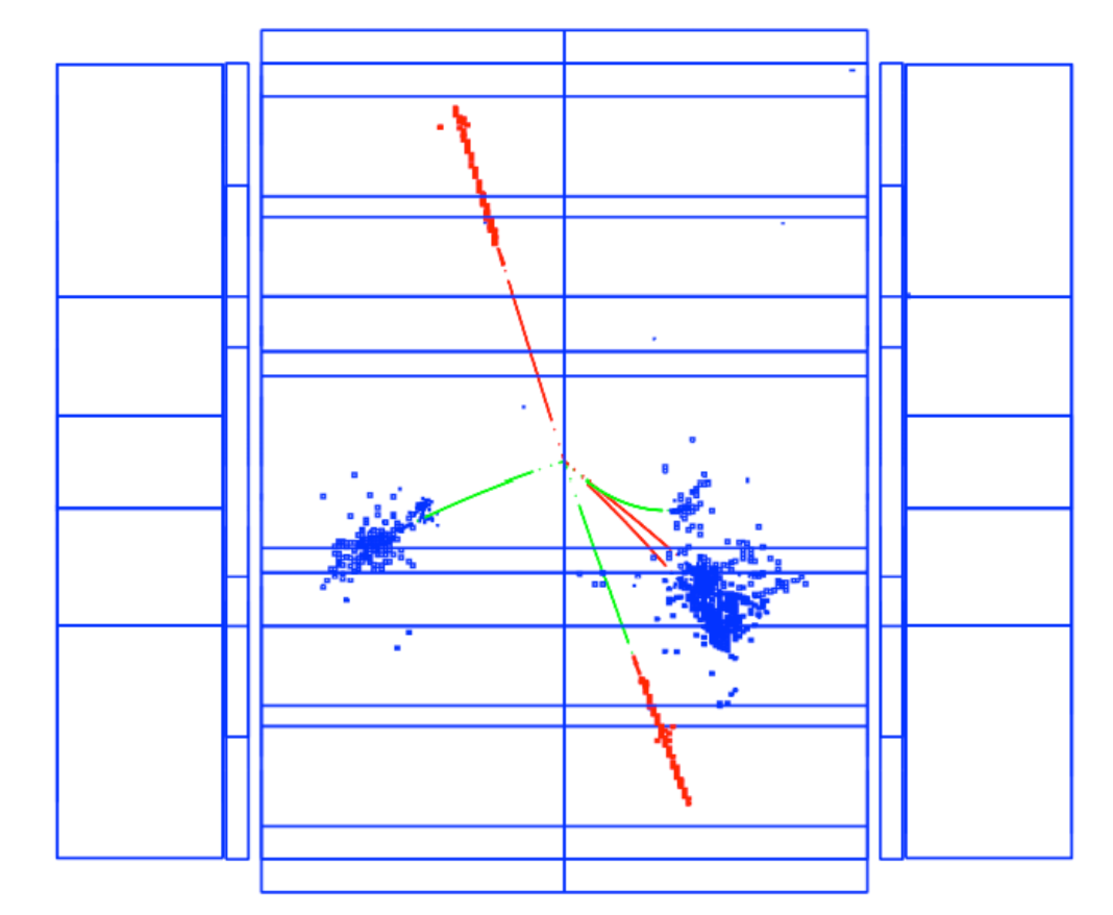
\includegraphics[width=0.5\hsize]{chapters/figures/htotautau.pdf}\ \ 
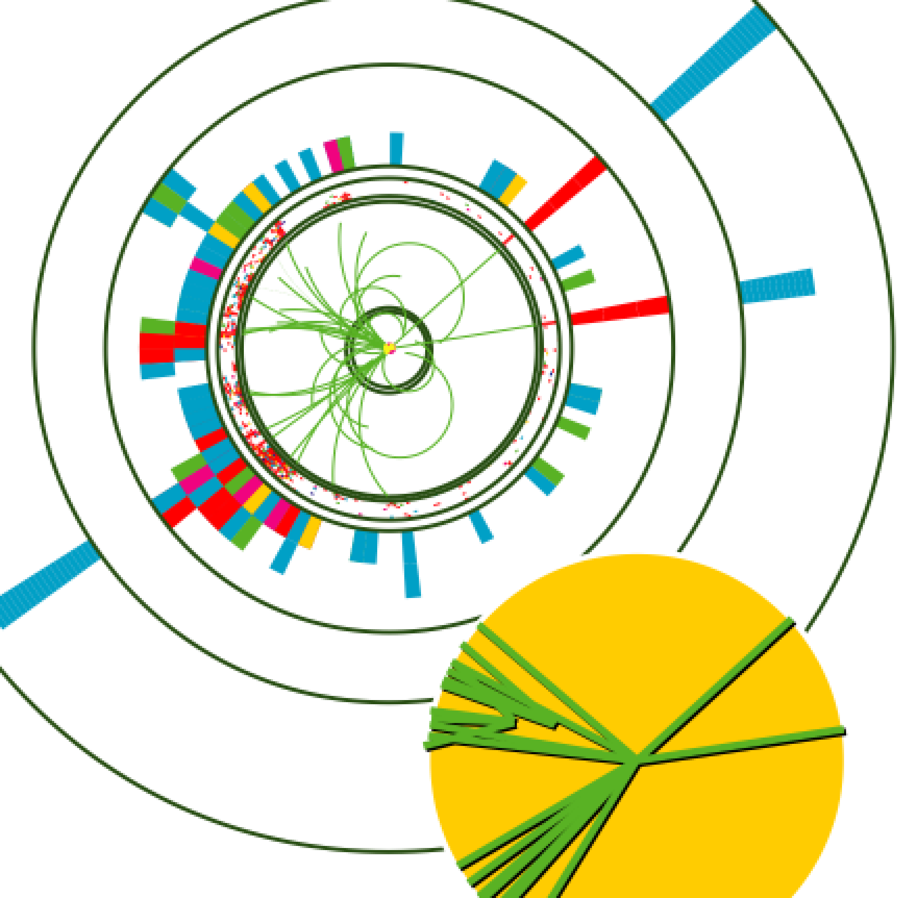
\includegraphics[width=0.40\hsize]{chapters/figures/htobb.pdf}
\end{center}
\caption{Event displays of $\ee\to ZH$ events  with $Z\to \mu^+\mu^-$, from full simulation: Left: $H\to \tau^+\tau^-$, ILC detector model;  Right: $H\to b\bar b$, SiD detector model.}
\label{fig:HiggsEvents}
\end{figure}
%%%%%%%%%%%%%%%%%%%%%%%%%%%%%%%%%%%%%%%%%%%%%%%%%%%%%%%%%%%%%%

\subsection{Search for exotic Higgs decays}

The fact that the reaction $\ee\to ZH$ yields {\it tagged} Higgs decays opens the 
possibility of another type of search for new physics.
The Higgs field is unique among SM fields in that it can form a dimension-2 operator 
$\Phi^\dagger \Phi$ with zero SM quantum numbers.  If there is any sector of fields that contains its own scalar field $\Sigma$, there will in general be a renormalizable coupling 
\beq
          \Delta \L   =   \eta\    (\Phi^\dagger \Phi) \, (\Sigma^\dagger \Sigma)  \ .
\eeq{Higgsportal}
The coupling constant $\eta$ is dimensionless, so the connection can be made at any (high) mass scale.   Thus it is possible for the Higgs boson to access a sector of elementary particles that have no other connection to the fields of the SM. 

If there is a new sector of particles with zero SM quantum numbers such that some of those particles have pair-production thresholds below 125 GeV, those particles should appear in Higgs boson decays.   If the particle that makes up cosmic dark matter is light enough to be produced in this way, the Higgs boson will have decays to invisible final states.   It is also possible that the new particles are unstable with respect to decay back to SM models.   Such decays could product  a number of different exotic
final states, including $4b$,
$4\tau$, $b\bar b$ + invisible states, and new particles with long lifetimes~\cite{Curtin:2013fra}.   With the data sample of the 250~GeV ILC, it is possible to search for all of these decay modes.   For  invisible Higgs decays, the expected 95\% CL exclusion limit on the  branching ratio is  $3\times 10^{-3}$, 
and for 
visible or partially visible modes the limits are in the range $10^{-3}$--$10^{-4}$~\cite{Liu:2016zki}. 

\subsection{Effective Field Theory framework for Higgs coupling determinations}
\label{subsec:phys_eft}

Though the goals of measuring the SM and exotic branching ratios of the Higgs boson are already very important, experiments at the ILC allow a further step.   The theory predictions described in Sec.~\ref{subsec:newphysicofH} refer to absolute partial decay widths.   These are 
related to the Higgs branching ratios by 
\beq
           \Gamma(H\to A\bar A) =   \Gamma_{tot} \cdot BR(H\to A\bar A)  \  .
\eeqn
The Higgs boson total width is very small---4~MeV in the SM---and it is not expected that any proposed collider can measure this value directly  with percent-level precision.
However, as we will now show, the ILC can determine the total width of the Higgs in a 
way that is highly model-independent and allows a 1\% absolute normalization of Higgs coupling constants.

A possible method to determine the Higgs width is to multiply each $HAA$ coupling by a parameter $\kappa_A$, and then fit these prarameters using data from $\ee\to ZH$.   In this simple method, the total cross section for $\ee\to ZH$ is proportional to $\kappa_Z^2$ and so the $\kappa_A$ parameters can be absolutely normalized.   This method has been used in much of the literature on Higgs coupling determinations, including \cite{Fujii:2015jha}.  In that paper, invisible and visible but exotic decay modes were treated by including these two partial widths as two additional parameters in the fit.  Using as inputs the measureable $\sigma\times BR$s for SM Higgs decay channels and Higgs decays to invisible final states, plus the total cross section for $\ee\to ZH$,  the ILC data would give a well-defined fit to the $\kappa_A$ parameters.

There are two problems with this method.  First, it is not completely model-independent.  Modelling the effects of new physics as a general set of dimension-6 operators as in \leqn{geneffL}, we find two different Lorentz structures for the modifications of the $HZZ$ vertex,
\beq
   \Delta \L =    (1 + \eta_Z) {m_Z^2\over v}  h Z_\mu Z^\mu + \zeta_Z {1\over 2v} h
   Z_{\mu\nu} Z^{\mu\nu} \ ,
\eeq{etazeta}
where $Z_\mu$ is the gauge field and $Z_{\mu\nu}$ is the field strength, 
and a similar pair of structures for the $HWW$ vertex.  In principle, the two coefficients  in each case should be independently determined from data.  Second, the method does not make the most effective use of the data set from $\ee$ colliders.  The total width of the Higgs boson is determined from the ratio  $\sigma(\ee\to ZH)/\Gamma(H\to ZZ^*)$.  Since the denominator is a 3\% branching ratio, this strategy sacrifices a factor 30 in 
statistics.

A much more effective method for fitting Higgs boson couplings is described in \cite{Barklow:2017suo}.   In this method, we model the effects of new physics by the most general set of dimension-6 operators that can appear in \leqn{geneffL}.  The complete set of $SU(3)\times SU(2)\times U(1)$-invariant lepton- and baryon-number conserving dimension-6 operators  includes 59 terms~\cite{Grzadkowski:2010es}.  However, for 
the analysis of $\ee$ collider data, we can restrict ourselves to electron reactions 
producing the Higgs boson and other color-singlet states.  Since there is a single SM effective
 Lagrangian that should apply to all processes, this method allows us to combine data on 
Higgs production with additional data sets from $\ee\to W^+W^-$ and precision electroweak
measurements.   It is also possible to make use of additional observables for Higgs production
beyond simple rates.  In particular, the angular distribution and polarization asymmetry in 
$\ee\to ZH$ play important roles.  These considerations give the method based on 
Effective Field Theory much more power in extracting the most accurate estimates 
of the 
Higgs boson couplings from the data.

It is sometimes considered a restriction that the EFT model contains only operators of dimension 6 without considering operators of dimension 8 and higher.    This means that the model will be somewhat inaccurate for the effects of new particles of mass close to 125~GeV.  However, one should remember that the effects of the top quark and the Higgs boson on precision electroweak observables are well-modeled by the $S$ and $T$ parameters~\cite{Peskin:1990zt}---which are induced at the level of the dimension-6 EFT---even though the masses of these particles are not far above the $Z$ mass.   Very light new particles can have a different effect, providing new Higgs decay channels and giving additional contributions to the Higgs width.  We take these possible effects into account explicitly in our global fit, as we will explain in Sec.~\ref{subsec:global:elements}.

After we describe the experimental methods and the expected measurement uncertainties for Higgs production in  Sec.~\ref{sec:higgs} and for $W$ pair production in Sec.~\ref{sec:ew},  we will present formal  projections for uncertainties in 
Higgs couplings in Sec.\ref{sec:global}, making use of the EFT  method.  Suffice it to say that the data set expected for the ILC at 250~GeV will  measure the $Hb\bar b$ couplings to 1\% accuracy, the $HWW$ and $HZZ$ couplings to better than 0.7\%, and the other 
major SM Higgs couplings to accuracies close to 1\%.    These measurements should be 
statistics-limited.  Above 250~GeV, a second Higgs production reaction, $\ee\to \nu\bar\nu h$ through $W$ boson fusion becomes important.  Using the additional data on $\ee\to ZH$ and the independent measurements from the $W$ fusion reaction, we expect that the uncertainties on Higgs couplings will decrease by another factor of 2. 


\subsection{$\ee \to W^+W^-$}
\label{subsec:phys_WW}
The reaction $\ee\to W^+W^-$ contributes to the analysis just described, but it has its own independent interest.  It has been appreciated for  a long time that this reaction provides an excellent way to test for the presence of dimension-6 operators that involve the $W$ and $Z$ fields.   The Feynman diagrams contributing to the reaction are shown in Fig.~\ref{fig:eeWWdiagrams}.   The process involves interference between $s$-channel diagrams with $\gamma$ and $Z$ exchanges and a $t$-channel diagram with neutrino exchange.  In the SM, there are large cancellations among these diagrams, but these are not respected by the dimension-6 contributions.   Thus, the dimension-6 coefficients appear in the cross section formulae enhanced by a factor $s/m_W^2$. 

%%%%%%%%%%%%%%%%%%%%%%%%%%%%%%%%%%%%%%%%%%%%%%%%%%%%%%%
\begin{figure}
\begin{center}
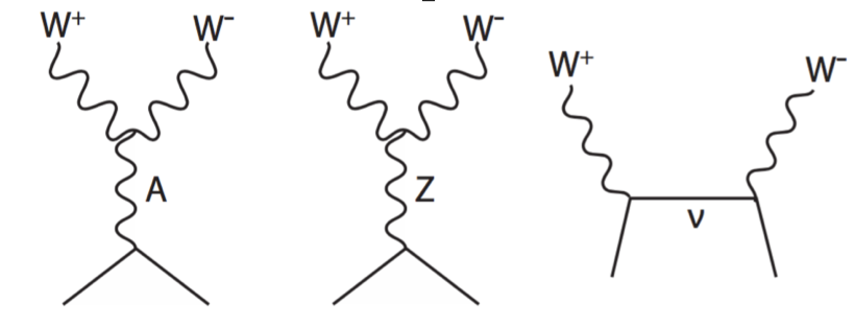
\includegraphics[width=0.80\hsize]{chapters/figures/WWdiagrams.pdf}
\end{center}
\caption{Feynman diagrams contributing to the process $\ee\to W^+W^-$ when contributing  dimension-6 operators are included.}
\label{fig:eeWWdiagrams}
\end{figure}
%%%%%%%%%%%%%%%%%%%%%%%%%%%%%%%%%%%%%%%%%%%%%%%%%%%%%%%%%%%%%%

The largest part of the dimension-6 effect can be described by shifts of the form 
factors for the $WW\gamma$ and $WWZ$ vertices.  These vertices can be parametrized as \cite{Hagiwara:1986vm}
\beqa
\Delta \L  &=& i g_V \biggl\{    V^\mu \bigl( { \hat W}^-_{\mu\nu}
W^{+\nu} -  {\hat W}^+_{\mu\nu}
W^{-\nu} \bigr)  +  \kappa_V  W^+_\mu W^-_\nu {\hat V}^{\mu\nu} \CR
& & \hskip 0.7in + {\lambda_V \over m_W^2}{\hat W}^-_\mu{}^\rho {\hat W}^+_{\rho \nu}
 {\hat  V}^{\mu\nu}  \biggr\} \ ,
\eeqa{WWgZvertex}
where $V = A$ or $Z$.
 In the SM, $g_{1A} = e$, $g_{1Z} = e s_w/c_w$ and the other coeficients are zero at the tree level.   The result $g_{1A} = e$ is exact due to the QED Ward identity.  The dimension-6 operator corrections generate a 3-parameter shift of the other 5 coefficients. These shifts can in principle be measured both at electron and at hadron colliders.  However, measurements in $\ee$ have  definite advantages.   First, it is possible to use final states with hadronic $W$ decays to determine the complete kinematics of each event and, using this information, to separate the production of 
transverse and longitudinal $W$ bosons.   Then, using beam polarization and $W$ final-state polarization, the 3 possible shifts of the form factors can be measured separately.   Second,  the greater intrinsic accuracy of measurements in $\ee$ give excellent results at a center of mass energies of 250--500~GeV.  At hadron colliders, 
the factor $s/m_W^2$ can be much larger, and one can take advantage of this by observing the reaction at $WW$ pair masses above 1~TeV.  However, this can lead to ambiguities due to the possible influence of dimension-8 operators, whose effects grow as $(s/m_W^2)^2$~\cite{Falkowski:2016cxu}. 

In Section VII  below, after describing the experimental study of $\ee\to W^+W^-$, we will show that the ILC at 250~GeV is expected to improve the precision of $W$ form factor measurements by an order of magnitude over expected results from the HL-LHC.




\subsection{$\ee\to f\bar f$}
\label{subsec:phys_ff}

Fermion pair production provides a search for new forces that couple directly to the electron.   At LEP and LHC, $\ee$ and $q\bar q$ annihilation are used as probes for new gauge bosons appearing in the $s$-channel and for signals of fermion compositeness. 

The comparison with LEP 2 is instructive.   The ILC will operate at an energy not so far above that of LEP 2  (250~GeV {\it vs.}  180--208~GeV)  but with much higher luminosity (2 ab$^{-1}$  {\it vs.} a total of 1~fb$^{-1}$ over 4 experiments).   For statistics-limited measurements, this gives a factor 
\beq
   \biggl[{  s \cdot \int \L |_{ILC}\over s \cdot \int \L|_{LEP}} \biggr]^{1/2} \approx 
                    60 
\eeqn
improvement in sensitivity to deviations from the SM, or an improvement of  7.5 in the mass scale that can be accessed.   Though the comparison depends on the particular model, this corresponds to the ability to observed new vector bosons at 5--6 TeV and 
contact interaction scales of 70~TeV, comparable to  the projected reach of the HL-LHC. 

 In addition, the information from ILC is very specific.   Measuring the cross section for $\ee\to f\bar f$ in the forward and backward directions for $e^-_L$ and $e^-_R$ beams gives four  different observables, each of which corresponds to a different dimension-6 effective  interaction.   Discovery of an anomaly points directly to a model interpretation, either with an $s$-channel resonance or with new interactions at higher energy.   This information can be put together with results of resonance searches at the LHC. 

The reaction $\ee\to b\bar b$ deserves special consideration. In models in which the Higgs boson is composite, typically either the $t_L$ or the $t_R$ must be composite also to generate a large enough $t$ quark mass.    The $b_L$ is the $SU(2)$ partner of the $t_L$ and so must have the same admixture of composite structure.    If it is the $t_R$ that is more composite, it is not required that the $b_R$ is composite, but this often happens in models.  This can generate few-percent corrections to the rates for $e^-_{L,R} e^+\to b_R\bar b_L$ at the ILC~\cite{Funatsu:2017nfm,Yoon:2018xud}.   It is possible that this effect, rather than effects in Higgs decays, would be the first indication of a composite Higgs sector. 

     
\subsection{Search for pair-production of new particles}

Despite the wide range of direct searches for new particle pair production at the LHC, 
those searches have blind spots corresponding to physically interesting models.  The two most important of these are:
\begin{enumerate}
\item  Insensitivity to new particles with electroweak interactions only that decay to an invisible partner with a mass gap of less than 5~GeV.   Though this case seems quite special, this is exactly the set of properties predicted for the charged Higgsino of SUSY models.  Dark matter scenarios involving coannihilation can also fall into this blind spot, since in those models there is an electroweak partner separated from the dark matter particle by $k_B T$ at the thermal dark matter freezeout temperature of 5-10~GeV.
\item Insensitivity to production of pairs of invisible particles observed through radiation of an initial-state gluon.   At the LHC, such ``mono-gluon'' events have as a background initial state radiation in the Drell-Yan process, and the sensitivity to such events is limited by the precision of our knowledge of the Drell-Yan cross section.
\end{enumerate}
In both cases, the ILC can detect these new physics events for particle masses almost up to half of  the collider center of mass energy.

The experimental aspects of these particle seaches are discussed in Section~VIII.  A broader review of the opportunities for new particle discovery at $\ee$ colliders can be found in \cite{Fujii:2017ekh}.

\subsection{The central role of beam polarisation}
\label{subsec:beampol}

One theme that runs through all of the analyses discussed in the following sections is the  important role of beam polarisation.   The use of beam polarisation may be unfamiliar to many readers, since all recently operated colliders -- the Tevatron, PEP-II and KEK-b, and the LHC -- have had unpolarised beams.   In hadronic 
collisions, the effects of polarisation are relatively small, first, because the dominant QCD interactions conserve parity and, second, because the proton is a composite particle, so high proton polarisation translates to much smaller polarisation for the constitutent quarks and gluons.   At a high-energy $\ee$ collider, the situation is very different.  The dominant interaction is the electroweak interaction, which has 
order-1 parity asymmetries in its couplings.  The beam particles are elementary, so that 80\% beam polarisation translates to 80\% polarisation in the colliding partons.
This implies  that polarisation effects are large at $\ee$  colliders and can be used to great advantage.   

It is very challenging to achieve high beam polarisation in circular colliders, especially for longitudinal polarisation.   Transverse beam polarisation was observed at LEP in single- and separated-beam operation but not for 
colliding beams~\cite{Assmann:1998qb}.  However,  a linear electron or positron
collider naturally preserves longitudinal beam polarisation.    The design of the 
ILC has been thought through  to produce, maintain, and control 
beam polarisation for both electrons and positrons, as has been explained in 
Sec.~\ref{par:beampol}.  This brings advantages for physics that we now discuss.

There are three major uses of beam polarisation in the experiments planned for ILC:
\begin{enumerate}
\item  Measurement of helicity-dependent electroweak couplings
\item Suppression of backgrounds and enhancement of signals
\item  Control of systematic uncertainties
\end{enumerate}
We discuss the first two of these points here.  The third, which is particularly 
important to claim a discovery from  precision measurements, is discussed in Sec.~\ref{subsec:polarisation}.  A comprehensive review of the role of polarisation with many more examples can be found in~\cite{MoortgatPick:2005cw}, and, for  positron polarisation in particular, in~\cite{Fujii:2018mli}. 

To begin, we need some notation. Let $P_{e^-}$ and $P_{e^+}$ be, respectively, the longitudinal polarisations of the electron and positron colliding beams, equal to $+1$ for completely polarised right-handed beams and $-1$ for completely polarised left-handed beams.   Let $\sigma_{RR}$, $\sigma_{RL}$, $\sigma_{LR}$, $\sigma_{LL}$ be the cross sections for a given process 
with completely polarised beams of the four possible orientations.  Since the electron has only two spin  states, the 
cross section for general beam  polarisations is given by 
\begin{eqnarray}
\sigma_{\Pem\Pep} &=& \frac{1}{4}\bigl\{
     (1+\Pem)(1+\Pep) \sigmaRR  \nonumber \\
&& + (1-\Pem)(1-\Pep) \sigmaLL \nonumber \\
&& + (1+\Pem)(1-\Pep) \sigmaRL \nonumber \\ 
&& + (1-\Pem)(1+\Pep) \sigmaLR \bigr\},
\label{eq:pol:xsec}
\end{eqnarray}

For $s$-channel $\ee$ annihilation processes, helicity conservation implies that only $\sigma_{RL}$ and $\sigma_{LR}$ are nonzero.
In this case Eq.~\leqn{eq:pol:xsec} reduces to the simpler form
\begin{equation}
 \sigma_{\Pem\Pep} = 2 \sigma_0 (\Leff/\mathcal{L}) \left[1 - \ALR \Peff \right]
\label{eq:pol:xsecschan}
\end{equation}
where $\sigma_0$ is the unpolarised cross section, and \Leff\ and \Peff\  
are the effective luminosity and polarisation, defined, respectively, as 
\begin{equation}
\Peff= \frac{\Pem - \Pep}{1 - \Pep\Pem}
\label{eq:def-leff-peff}
\quad\mbox{\rm and }\quad
\Leff=\frac{1}{2}(1 -\Pep\Pem)\L \ . 
\end{equation}
The coefficient $\ALR$ is the intrinsic left-right asymmetry of the reaction cross section,
\beq
  \ALR =    {\sigmaLR - \sigmaRL\over \sigmaLR + \sigmaRL } \ . 
\eeq{eq:def-ALR}

In the electroweak interactions, it is typical that left-handed fermions have larger coupling constants than right-handed fermions.   Then, choosing $\Pem$ to be left-handed (negative) and $\Pep$ to be right-handed (positive) can confer important advantages.
Consider, for example, the typical ILC values $\Pem = -80\%$, $\Pep = +30\%$.    Then the effective polarization 
Eq. \leqn{eq:def-leff-peff} for the measurement of $\ALR$ values is  $\Peff = 90\%$.   The Higgsstrahlung process has a rather small polarisation asymmetry, $\ALR = 0.151$. Still, the luminosity is enhanced from the unpolarised case by  $ 40\%$. 

Such substantial values of the beam polarisations can be applied to physics measurements in the following ways:
\begin{itemize}
\item In $\ee\to f\bar f$, the $e^-_L$ and $e^-_R$ couple to different linear combinations of the $s$-channel $\gamma$ and $Z$
propagators.  Beam polarisation allows us to measure the couplings to these vector bosons independently.  In addition, an $s$-dependent change in the polarisation asymmetry can signal the presence of a new $s$-channel resonance.  
\item Similarly, in $\ee\to W^+W^-$, the separation of $\gamma$ and $Z$ couplings can be combined with information from the $W$ production angle and polarisations to completely disentangle the 14 complex parameters (28 real parameters) in the most general 
Lagrangian for triple gauge vertices.
\item In $\ee\to ZH$, measurement of  the polarisation asymmetry plays an important role in disentangling the various of  parameters 
that enter the EFT analysis of Higgs boson couplings.
\item If new particles are discovered in pair-production at the ILC, measurement of the production cross section with different beam polarisation settings allows their electroweak quantum numbers to be determined unambiguously.
\end{itemize}
We will present all of these applications in the sections to follow.

%%%%%%%%%%%%%%%%%%%%%%%%%%%%%%%%%%%%%%%%%%%%%%%%%%%%%%%%%%%%%%%%%%%%%%%
\begin{figure}
\centering
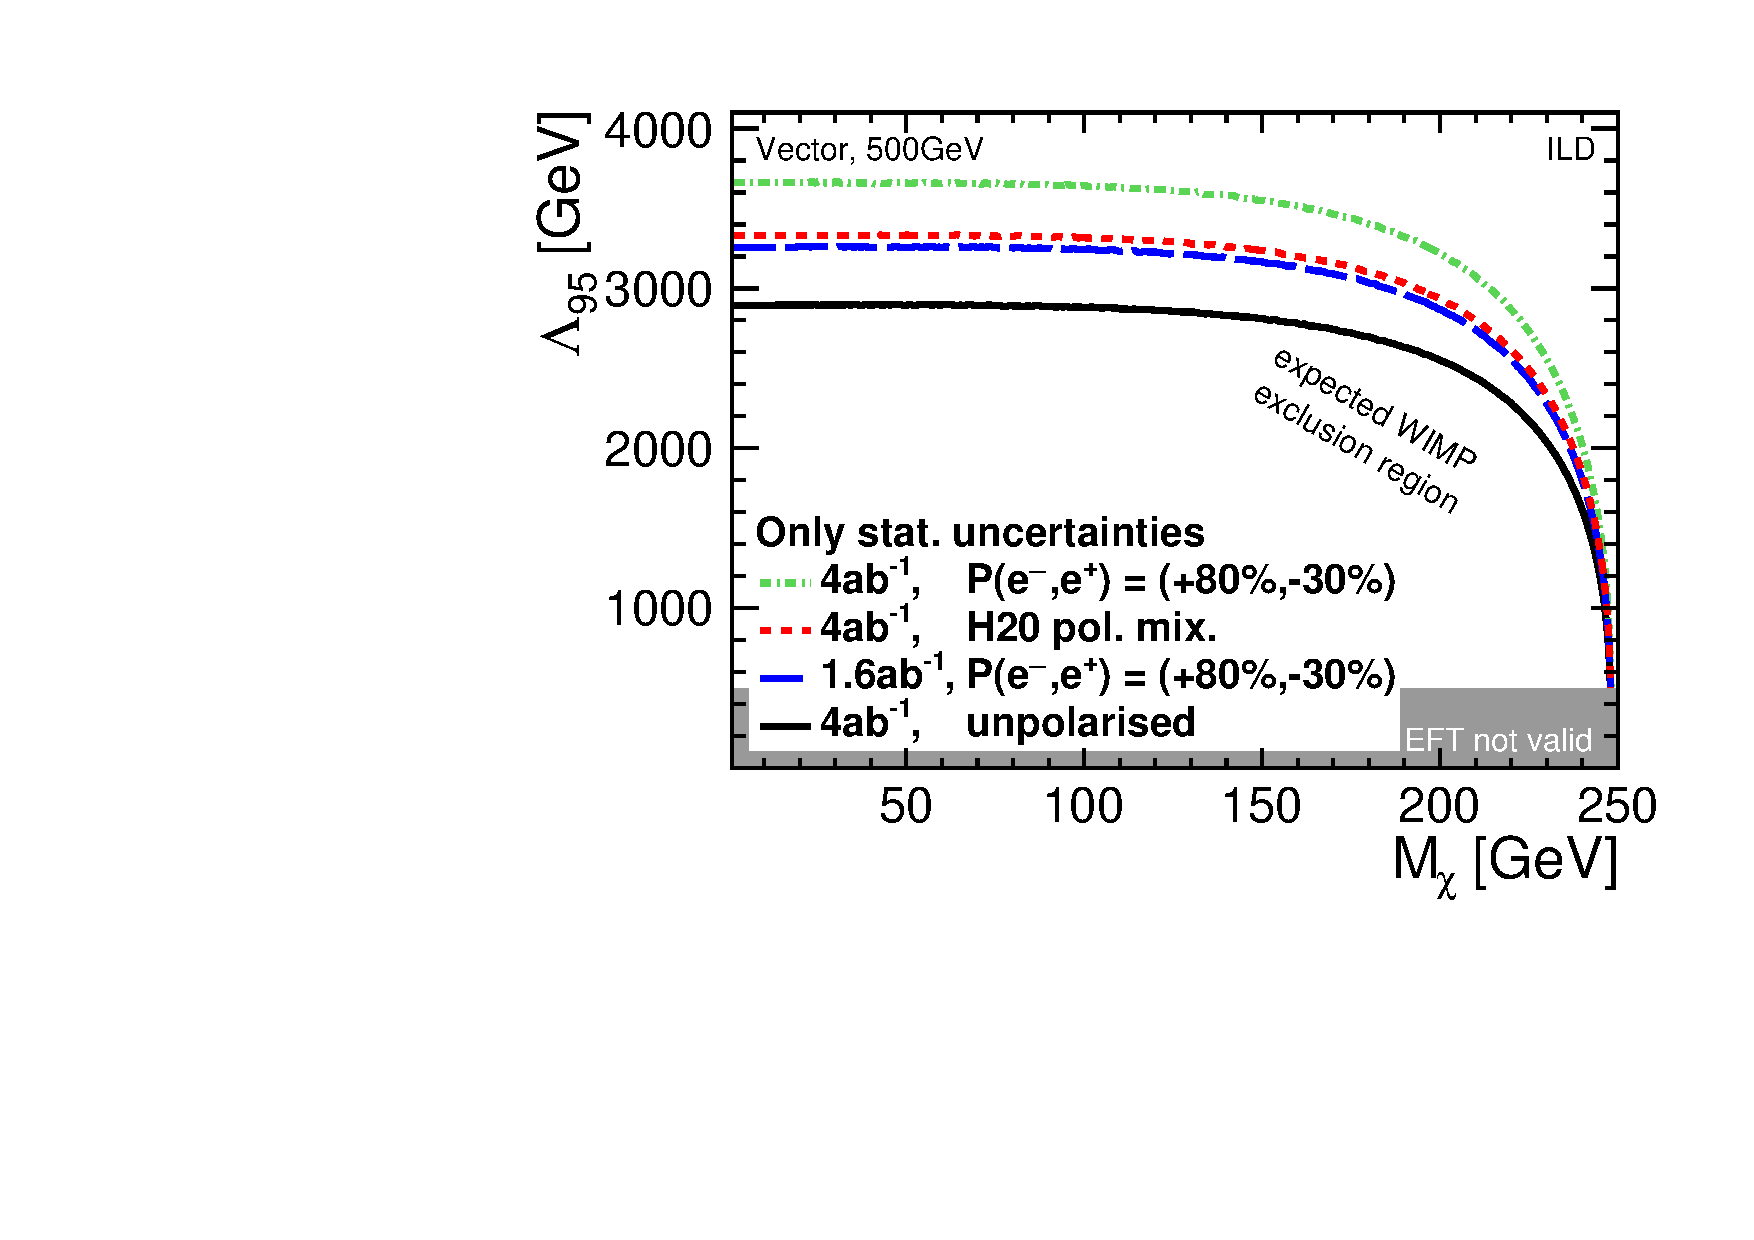
\includegraphics[width=0.95\linewidth]{./chapters/figures/vector_noSystematics.pdf}
		
\caption{Comparison of the 95\% confidence lower limit on the mediator scale for dark matter production using  the mono-photon channel,  for different assumptions on luminosity and polarisation.  See Sec.~\ref{sec:searches} for a description of the analysis~\cite{Habermehl:417605}. Note that this plot considers {\em statistical uncertainties only}. The corresponding comparison {\em including systematic uncertainties} is shown in Fig.~\ref{fig:polWIMPsys}.}
\label{fig:polWIMPstat}
\end{figure}

%%%%%%%%%%%%%%%%%%%%%%%%%%%%%%%%%%%%%%%%%%%%%%%%%%%%%%%%%%%%%%%%%%%%%%%%%%%%5


It is also possible to take advantage of differences in the polarisation effects on signal and background cross sections to enhance signals and control backgrounds.  Unlike annihilation processes, radiative Bhabha scattering and 2-photon processes have nonzero $\sigma_{LL}$ and $\sigma_{RR}$, so it is possible to test strategies for the suppression of these backgrounds using  data sets with
in which $\Pem$ and $\Pep$ have the same sign.   The reaction $\ee\to W^+W^-$ has a relatively large cross section among 
annihilation processes and so is often the dominant background to studies of or searches for other processes.   However, this process also has a large polarisation asymmetry, with $\sigma_{LR}/\sigma_{RL} \approx 30$.  Then running with $\Pem = +80\%$, $Pep = -30\%$ essentially turns off this background.   

As an example of the effectiveness of background suppression, we show in Fig.~\ref{fig:polWIMPstat} a comparison of searches  for invisible dark matter particles $\chi$  in the mono-photon  mode $\ee\to \gamma+ \chi\chi$ under different assumptions on luminosity and polarisation.   The predicted 95\% confidence lower limit on the mediator scale $\Lambda_{95}$ is shown as a function of 
the $\chi$ mass.  Of course, the polarisation settings cannot be simultaneously optimized for each physics analysis.  But the figure
shows that a data set of 1.6~\iab\ with optimal polarisation is considerably more powerful than a data set of 4~\iab\ with unpolarised
beams.  The red dotted curve shows the result for the H20 scenario with polarisations given in Tab.~\ref{tab:pollumirel}.   For clarity, the  figure includes statistical errors only. 

The influence of polarisation on systematic errors is equally important.  Where experiments with unpolarised beams give one measurement, experiments with both electron and positron beams polarised give 4 independent measurements.  These can be used as cross-checks for  the understanding of systematics, and also to form combinations in which the 
dominant systematic errors cancel.  We will 
discuss this point in more detail in Sec.~\ref{subsec:polarisation}.